\documentclass{article}

\usepackage[french]{babel}
\usepackage[latin1]{inputenc}
\usepackage[T1]{fontenc}
\usepackage[]{algorithm2e}
\usepackage{graphicx}
\usepackage{float}

%%%%%%%%%%%%%%%% Lengths %%%%%%%%%%%%%%%%
\setlength{\textwidth}{15.5cm}
\setlength{\evensidemargin}{0.5cm}
\setlength{\oddsidemargin}{0.5cm}

%%%%%%%%%%%%%%%% Variables %%%%%%%%%%%%%%%%
\def\projet{4}
\def\titre{Non-linear systems of equations - Newton-Raphson method}
\def\groupe{4}
\def\equipe{5}
\def\responsible{mbounakhla}
\def\secretary{gzahar}
\def\others{rboudjeltia, lcidere, pgaulon}

\begin{document}

%%%%%%%%%%%%%%%% Header %%%%%%%%%%%%%%%%
\noindent\begin{minipage}{0.98\textwidth}
  \vskip 0mm
  \noindent
  { \begin{tabular}{p{7.5cm}}
      {\bfseries \sffamily
        Project n�\projet} \\ 
      {\itshape \titre}
    \end{tabular}}
  \hfill 
  \fbox{\begin{tabular}{l}
      {~\hfill \bfseries \sffamily Group n�\groupe\ - Team n�\equipe
        \hfill~} \\[2mm] 
      Responsible: \responsible \\
      Secretary: \secretary \\
      Programmers: \others
    \end{tabular}}
  \vskip 4mm ~

  ~~~\parbox{0.95\textwidth}{\small \textit{Abstract~:} \sffamily 
 }
  \vskip 1mm ~
\end{minipage}

%%%%%%%%%%%%%%%% Main part %%%%%%%%%%%%%%%%
\section*{Newton-Raphson method}
To begin with, the Newton-Raphson algorithm had to be programmed in order to solve all the non-linear problems given. This algorithm is based on the equation $f(U+V)=0$ in which $f(U+V)$ can be approximated by $f(U) + H(U) \times V$. In this equation, $f$ is a differentiable function $\mathbf{R}^m \rightarrow \mathbf{R}^n$, $H$ is the Jacobian matrix of function $f$, $U$ is the vector representing the current position and $V$ represents the next position approaching a root of function $f$. Subsequently the relation linking $H$, $f$, $U$ and $V$ could be immediately deduced: $f(U)+H(U) \times V = 0$ or in other words $H(U) \times V = -f(U)$.

As numpy.linalg.lstsq is based on a SVD decomposition, its complexity is approximately $\theta(n^3)$ where $n$ is the size of the $J$ matrix. Therefore in the worst case, the Newton-Raphson algorithm has a complexity measured by $\theta(N \times n^3)$, so a cubic complexity.

Here is a Newton-Raphson algorithm including backtracking:

\begin{center}
  \begin{algorithm}[H]
    \KwData{a function $f$, it's Jacobian matrix $J$, a starting vector $U0$, an iteration maximum number $N$, a convergence measurement $epsilon$}
    \KwResult{a root of the function $f$}
    $U \leftarrow U0$\;
    $i \leftarrow 0$\;
    \While{ $(i < N)$ and $(||f(U)|| >= epsilon)$}{
      $V \leftarrow$ Solution($J(U) * V + f(U) = 0$)\;
      \While{$||f(U+V)|| >= ||f(U)||$}{
        $V \leftarrow V/2$\;
      }
      $U \leftarrow U+V$\;
      $i \leftarrow i+1$\;    
    }
    \Return U\;
    \caption{Newton-Raphson algorithm with backtracking}
  \end{algorithm}
\end{center}

Backtracking prevents this algorithm from overlooking solutions. If the $f(U+V)$ value goes too far, backtracking forces this value to go back. Here, the choice of going back with a half step was made.
  
The second While loop is the code portion including backtracking. Without it, this algorithm is the simple Newton-Raphson one. For each calculus using Newton-Raphson, two graphs were calculated, representing the $||f(U)||$ value according to the iteration number. The first one was for the algorithm without backtracking and the second one with backtracking. But both graphs were the same. We supposed that there were not enough iterations in these calculi to tell the difference. So for these calculi, either algorithm can be used without any difference.
\begin{center}
  \begin{figure}[H]
    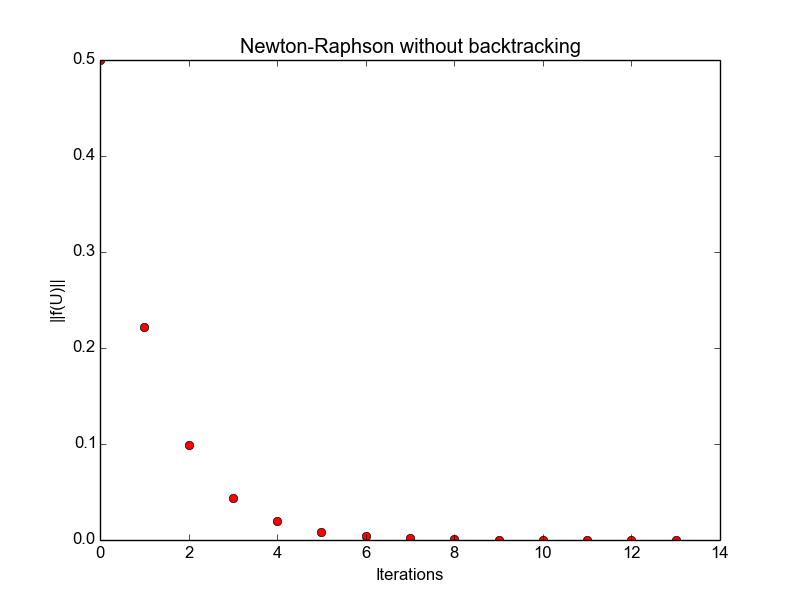
\includegraphics[scale=0.3]{Newton-Raphson_no_backtracking.png}
    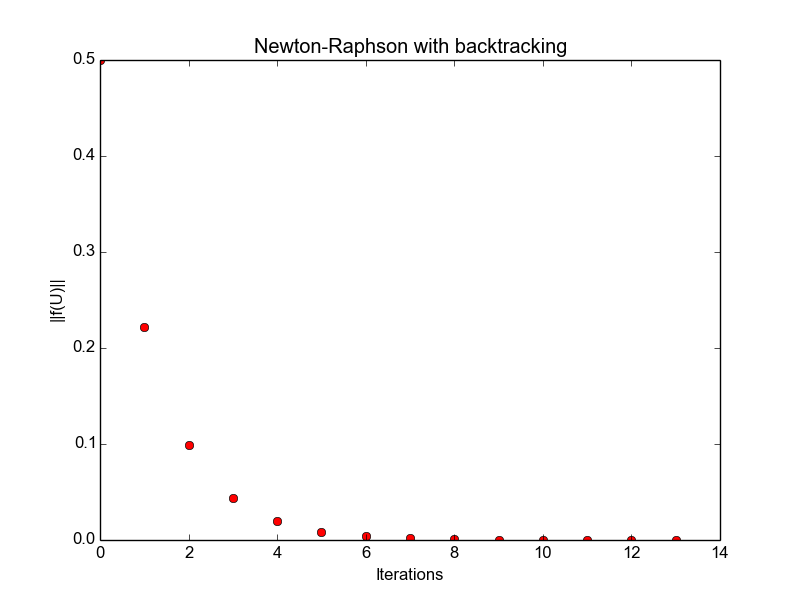
\includegraphics[scale=0.3]{Newton-Raphson_backtracking.png}
    \caption{Convergence comparison between the Newton-Raphson algorithm without backtracking and with backtracking}
  \end{figure}
\end{center}

\section*{Computation of the Lagrangian points}
The Lagrangian points are the five equilibrium points in an orbital configuration.
The configuration chosen was the one including the Sun and the Earth. So there were two masses. The first one, representing the Sun, a hundred times as heavy as the second one, the Earth, and they were separated by a certain distance called radius symbolized R.

In order to solve this problem, the first step was to modelize the different forces: elastic, gravitational and centrifugal. Subsequently, to obtain the first three Lagrangian points, the Newton-Raphson method was used three times to obtain each root of each equilibrium equation. The last two points were calculated geometrically.

\begin{center}
  \begin{figure}[H]
    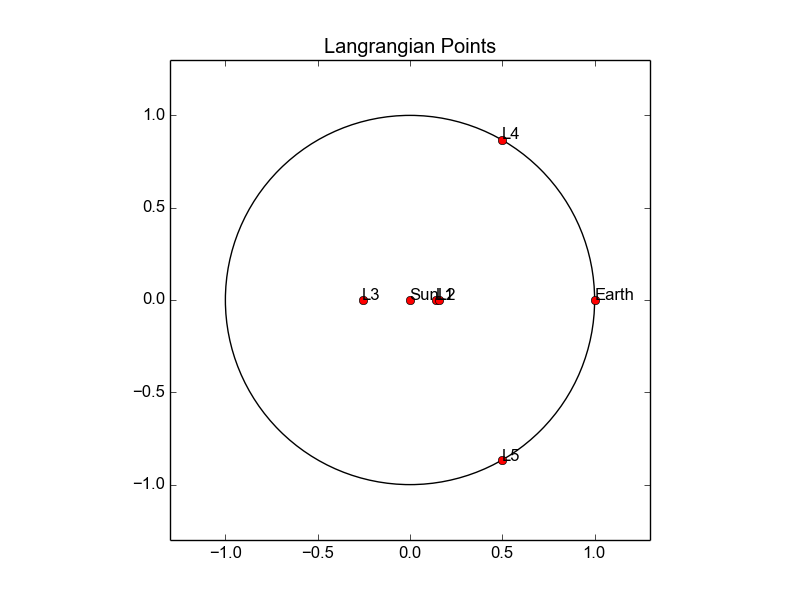
\includegraphics[scale=0.35]{Lagrangian_Points.png}
    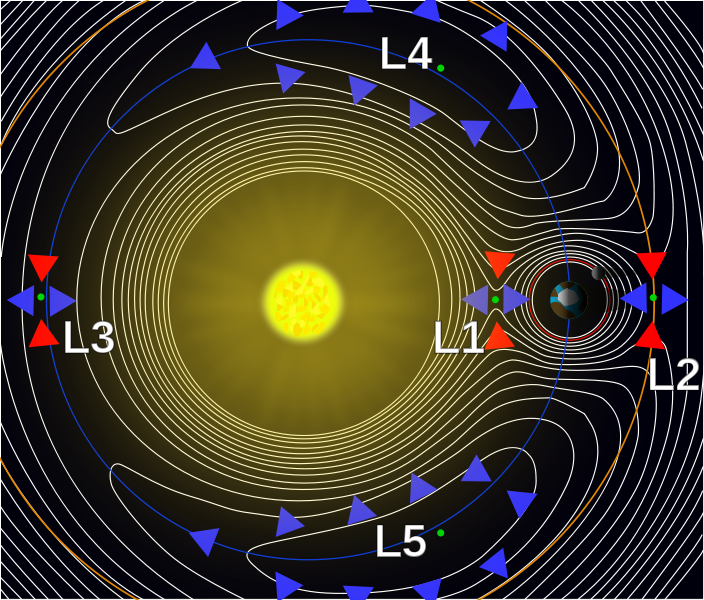
\includegraphics[scale=0.2]{Lagrangian_Points_Wiki.png}
    \caption{Comparison between our solution and the solution on Wikipedia's website}
  \end{figure}
\end{center}

In this situation it was possible to calculate the five Lagrangian points. But the solutions we found were lower than expected. The first three points should have been a little bit further from the Sun, with a distance approximately that of R. We did not find the reason for this problem. We suspected that there was a wrong equilibrium formula or a wrong derivative of this formula, or bugs in our Newton-Raphson algorithm, or even our way of using it could have been wrong. But investigating each of these possibilities did not lead to a satisfactory solution.

\end{document}
